User profiles on photosharing networks often contain a significant amount of photos tagged with latitude-longitude GPS locations. Over time the accumulated location data can build up to comprehensive mobility profiles. Based on this insight and given that many user profiles on photosharing networks are publicly accessible we now introduce a methodology and its application to construct mobility datasets from readily available data. An overview of our methodology is shown in Figure~\ref{fig:system}. 

\begin{figure}[h]
	\begin{center}
		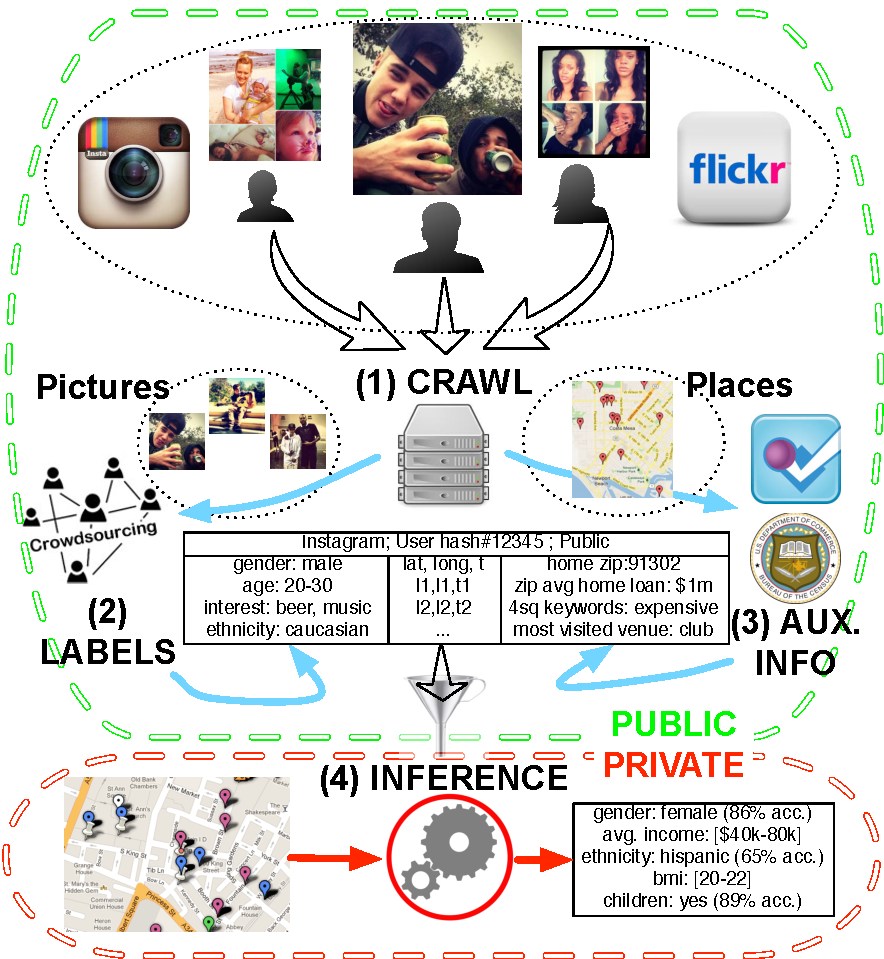
\includegraphics[width=\linewidth]{fig/footprints/system.pdf}
	\end{center}
	\caption{Methodology overview. A mobility dataset can be built in the following steps: (1) Public user profiles of a photosharing service are crawled and photo metadata are extracted into a database (Data Collection). (2) Corresponding photos are labeled (with labels for ethnicity, gender, etc.) by crowd workers in an online labor marketplace (User Labeling). (3) The dataset is further enhanced with auxiliary data, e.g., with the information that a certain location is close to a restaurant (Adding Auxiliary Information). (4) The dataset can then be used to analyze attributes on various demographic levels or train and test classifiers for individual inferences.}
	\label{fig:system}
\end{figure}

\paragraph{Data Collection} 
%\textbf{Data Collection.} 
Applying this methodology, we collected publicly available photo metadata from Instagram covering data for the years from 2011 through 2013. This data collection and use was exempt from user informed consent under our institution's IRB rules since (1) we only collected publicly available online metadata, (2) after we used the metadata and the users were labeled, any identifying information, such as usernames, were removed, and (3) we only kept track of users' identities separately and for one single purpose (ensuring that the data we collected still belongs to a public Instagram  profile). We started our crawl from a root user (the founder of Instagram, on whose feed a large and diverse group of users comment) and followed further users subsequently through comments and likes. We skipped users with no geotagged photo in their first 45 photos. Our crawl retrieved a total of 35,307,441 photo location points belonging to 118,374 unique users.

\paragraph{User Labeling} 
%\textbf{User Labeling}.
To match previous studies~\cite{Isaacman:2011un,Isaacman:2011cn,Isaacman:2010en} that leveraged ZIP codes of CDR billing addresses from the Los Angeles (LA) and New York City (NY) metropolitan areas we randomly chose users from those areas as well. A user's home is the ZIP code where he or she had the most checkins (that is, photos taken). Note that this mitigates the content produced by tourists and other occasional visitors to LA and NY unless those have no other Instagram activity. A combination of workers on Amazon Mechanical Turk (MTurk) and undergraduate students were asked to annotate users' ethnicities and gender based on the users' photos. However, in order to ensure that user pictures on Instagram profiles are sufficient to make a conclusive determination of users' ethnicities and genders we ran a preliminary experiment by selecting 200 profiles at random (excluding celebrities and business accounts) and having each labeled independently by two undergraduate students. We observed a strong agreement on gender (98\%). The errors corresponded to a family profile belonging to multiple people and profiles with one picture.

For ethnicity labeling we leveraged Census categories. We asked the student annotators to categorize each user either as Hispanic or Latino (Hispanic), White alone (Caucasian), Black or African American alone (African American), or Other (combining all remaining Census categories, including Asian). Merging all remaining Census fields in the last category limits our detail view, although we would otherwise have some annotations being quite rare. Just as in the Census, our Hispanic category includes Hispanics and Latinos of any race, while the remaining categories do not include any Hispanics or Latinos. We found that our profiles are diverse: 45\% Caucasian, 21\% Hispanic, 15\% African American, and 19\% Other. The students' labels matched 87\% of the time and when evaluated as a binary classification task (Caucasian vs. all other categories) the agreement reached 94\%. It should be noted that the two labeling students were of different gender and ethnicity themselves. In conclusion, despite sparse data and ethnicity spanning a continuous spectrum, we found that labels are surprisingly predictable and consistent across annotators. As studies confirmed that 91\% of teens post a photo of themselves on social networks~\cite{PewTeen} and that 46.6\% of photos are either selfies or show the user posing with other friends~\cite{ICWSM148118} there is also evidence in many cases that it is actually the account owner who is shown in the pictures.

\begin{figure}[htp]
	\centering
	\begin{subfigure}[t]{1.22in}
		\centering
		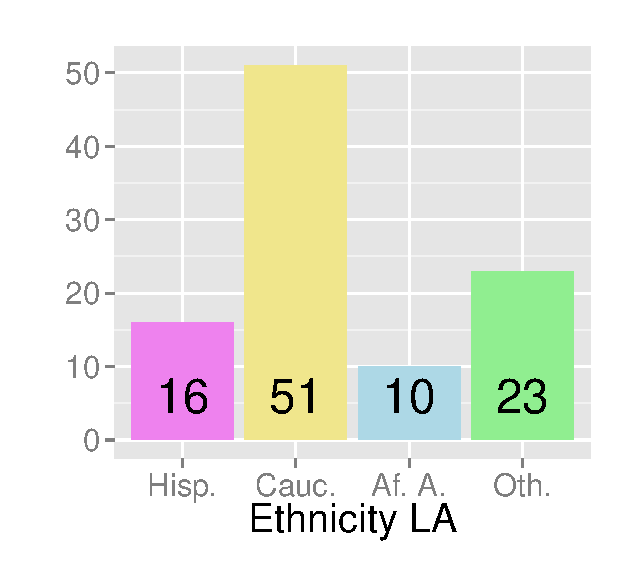
\includegraphics[width=1.22in]{fig/footprints/la_eth_bar.eps}
	\end{subfigure}
	\begin{subfigure}[t]{1.22in}
		\centering
		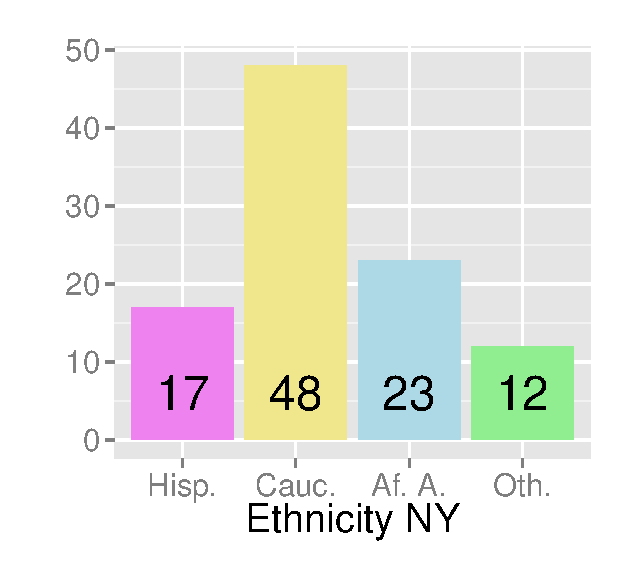
\includegraphics[width=1.22in]{fig/footprints/ny_eth_bar.eps}
	\end{subfigure}
	\begin{subfigure}[t]{0.76in}
		\centering
		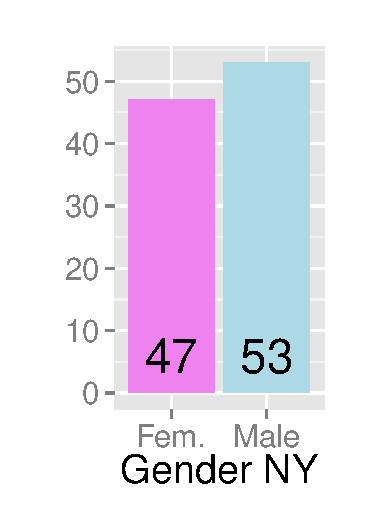
\includegraphics[width=0.76in]{fig/footprints/ny_gender_bar.eps}
	\end{subfigure}
{\small
\begin{tabular}{| l | c | c | c |}
\hline
                          & {\textit{Ethnicity LA}} & {\textit{Ethnicity NY}} & {\textit{Gender NY}} \\ \hline
{\textit{Users (n)}}      & 427                     & 588                     & 241 \\ \hline
K.'s $\alpha$ Multi.      & \textbf{0.74}           & \textbf{0.68}           & -   \\ \hline
K.'s $\alpha$ Binary      & \textbf{0.78}           & \textbf{0.74}           & \textbf{0.85} \\ \hline
\end{tabular}
}
\vspace{0.7ex}
	\caption{Annotations for LA and NY. Top: percentages of user labels for the different categories. Bottom: absolute numbers of labeled users and annotation agreement results.}
	\label{fig:demographics}
\end{figure}

To scale our annotation, we asked MTurk annotators to label a larger number of profiles for the same metropolitan areas using the same label categories. For consistency, we did not reuse the profiles used for the preliminary experiment described above. Each profile was labeled by two MTurk annotators. In cases of disagreement between the MTurk annotators we asked one of our undergraduate annotators for an additional label to break the tie or assign a label from a different third category. We decided to use a tiered annotation mechanism with the undergraduate annotator making the final decision in case of disagreements as unsupervised crowd workers on MTurk or similar platforms tend to be less attentive than physically available workers~\cite{Paolacci10runningexperiments}, who also have the possibility to ask clarifying questions. We were also careful to not drop any labels to avoid the introduction of a systematic annotation bias. Over two days 117 MTurk annotators participated in our task resulting in 1,015 properly labeled users with the labels shown in Figure~\ref{fig:demographics}. On the first day the annotators were compensated \$0.10 per annotation and on the second day \$0.05. The undergraduate annotator was compensated the regular stipend at our institution.

In order to measure the quality of agreement among the annotators we made use of Krippendorff's $\alpha$~\cite{Krippendorff}. Generally, values above 0.8 are considered as good agreement, values between 0.67 and 0.8 as fair agreement, and values below 0.67 as dubious~\cite{Manning:2008:IIR:1394399}. Figure~\ref{fig:demographics} shows that we obtained fair and good agreement and, thus, reliable ground truth for both our ethnicity and gender classifications. 

\paragraph{Adding Auxiliary Information}
%\textbf{Adding Auxiliary Information}.
We collected auxiliary information from two sources. First, for the comparative analysis of demographic patterns with our data in \S\ref{sec:demographic-patterns} we used data from the Census~\cite{census:2010} to associate geographic regions with gender and ethnicity distributions. 
Throughout the study we use Census-defined geographic granularities, ranging from block groups of 600-3k people to neighborhood tabulation areas (NTAs; 15k people), public use microdata areas (PUMAs; 100k people), and counties with populations of up to 2.6 million.
We adjusted the distributions by ethnicity- and gender-specific Internet \cite{file:2013,PewSocialMedia2012} and Instagram \cite{Pew2012} usage numbers. As explained in~\S\ref{sec:demographic-patterns} we also took into account that Caucasian Hispanics are often perceived as Caucasian alone~\cite{MelaninMillennium}. Second, for each checkin we obtained Foursquare information on the ten closest venues. We then used Foursquare's average venue popularities and venue categories as features for our inference algorithms (\S\ref{sec:inference}) since those features could provide an estimate of the types of places a user would visit.
